\documentclass[paperwidth=46in, paperheight = 33.11in]{baposter}%,draft,draft
% need to reference python libraries (numpy-stl, trimesh, glumpy, and etc.)

\usepackage{amsmath,amsbsy,amsfonts,amscd,mathtools} %

\usepackage{graphicx}
\graphicspath{{./diagrams/}}
\usepackage{epstopdf} %autoconvert eps inclusions to pdf
\usepackage{relsize}


\usepackage[export]{adjustbox} %enables the adjincludegraphics command, which lets me use unit-less clipping of images.

\usepackage{wrapfig}


\usepackage{tabularx} \newcolumntype{C}{>{\centering\arraybackslash}X}

\definecolor{bordercol}{RGB}{237,172,26}
 \definecolor{headercol1}{RGB}{237,172,26}
 \definecolor{headercol2}{RGB}{43,62,133}
 \definecolor{headerfontcol}{rgb}{1,1,1}
 \definecolor{boxcolor}{cmyk}{0,0,0,0}
 \definecolor{bgyellow}{cmyk}{0.004,0.004,0.044,0}
 \definecolor{bgblue}{cmyk}{0.068,0.013,0.023,0}



% Previous colors backup
% \definecolor{bordercol}{cmyk}{0,0.04,1,0.3}
%  \definecolor{headercol1}{cmyk}{0.0,0.18,1,0.15} 
%  \definecolor{headercol2}{cmyk}{1.0,0.64,0.0,0.60} 
%  \definecolor{headerfontcol}{rgb}{1,1,1}
%  \definecolor{boxcolor}{cmyk}{0,0,0,0}
%  \definecolor{bgyellow}{cmyk}{0.004,0.004,0.044,0}
%  \definecolor{bgblue}{cmyk}{0.068,0.013,0.023,0}



\usepackage[superscript,biblabel]{cite}


% adjust the separation between items in an enumeration or itemization
\usepackage[]{enumitem}
\setitemize{itemsep=2pt,align=left, leftmargin=*}
\setenumerate{itemsep=2pt,leftmargin=*,align=left}

\newcommand{\C}{\mathbb{C}}
\newcommand{\R}{\mathbb{R}}

\usepackage{helvet} %to use helvet font

\usepackage{hyperref}
\begin{document}

%%% Setting Background Image %%%%%%%%%%%%%%%%%%%%%%%%%%%%%%%%%%%%%%%%%%%%%%%%%%
%\background{
%	\begin{tikzpicture}[remember picture,overlay]%
%	\draw (current page.north west)+(-1em,1em) node[anchor=north west]
%	{\includegraphics[width=1.155\textwidth]{crystalbackground.jpg}};%
%	\end{tikzpicture}
%}

\begin{poster}{
%%%%%%%%%%%Poster Settings%%%%%%%%%%%%%
grid=false,
eyecatcher=true,
borderColor=bordercol,
headerColorOne=headercol1,
headerColorTwo=headercol2,
headerFontColor=headerfontcol,
boxColorOne=boxcolor, %simple, non-gradient color, so ColorTwo not needed
headershape=rounded, %shape of upper corners
headerfont=\Large\sffamily\bfseries,%  headers are sans serif, bold, and large.  this overrides the serif helvet font which would otherwise be used.
textborder=rounded, %roundedright
bgColorOne=bgyellow,  %these colors are named above in the header.
bgColorTwo=bgblue, %for gradient background
background=shadeLR,
headerborder=closed,
boxshade=plain,
headerheight=3cm,
columns = 7,
}
%%%%%%%%%%%%% Eye Catcher %%%%%%%%%%%%%%
{
%Eye Catcher, empty if option eyecatcher=false - unused
    
\includegraphics[height=1.0in]{Power-of-AND_stckd_blu_CMYK.eps}

}
%%%%%%%%%%%%% Poster title %%%%%%%%%%%%%
{\sffamily\bfseries \fontsize{22pt}{12pt}\selectfont \vspace{1.5mm}
3D Visualization of Algebraic Surfaces Using Bertini\_real, Python and Blender
}
%%%%%%%%%%%%% Authors %%%%%%%%%%%%%%%%%%
{
\begin{minipage}{1\linewidth} \bf\sf
\centering
\footnotesize{
\begin{tabularx}{0.99\linewidth}{C  C  C} 
\Large{\sffamily\bfseries Foong Min Wong}			&	\Large{\sffamily\bfseries Dan Hessler}      & \large{Danielle Brake, PhD}\\
wongf3284@uwec.edu & hessledd3607@uwec.edu & brakeda@uwec.edu \\
%University of Notre Dame ACMS 	&	Colorado State University Mathematics	&   Mathematical Biosciences Institute &	University of Notre Dame ACMS	& University of Notre Dame ACMS &General Motors R\&D   \\
%dbrake@nd.edu & & & & &
\end{tabularx}}
\end{minipage}
\centering
\newline
\newline
\large{\sffamily Department of Mathematics, University of Wisconsin -- Eau Claire}
}
%%%%%%%%%%%% Logo %%%%%%%%%%%%%%%%%%%%%%
{

\includegraphics[width=2in]{UWEC-stacked-wordmark-Blue_cmyk.eps} 
}

%%%%%%%%%%%% Begin Boxes %%%%%%%%%%%%%%%

\headerbox{Research goals}{name=goals, column = 0, row = 0,span=2}{

\begin{center}

\begin{minipage}[t]{0.48\linewidth}
    \begin{center}
        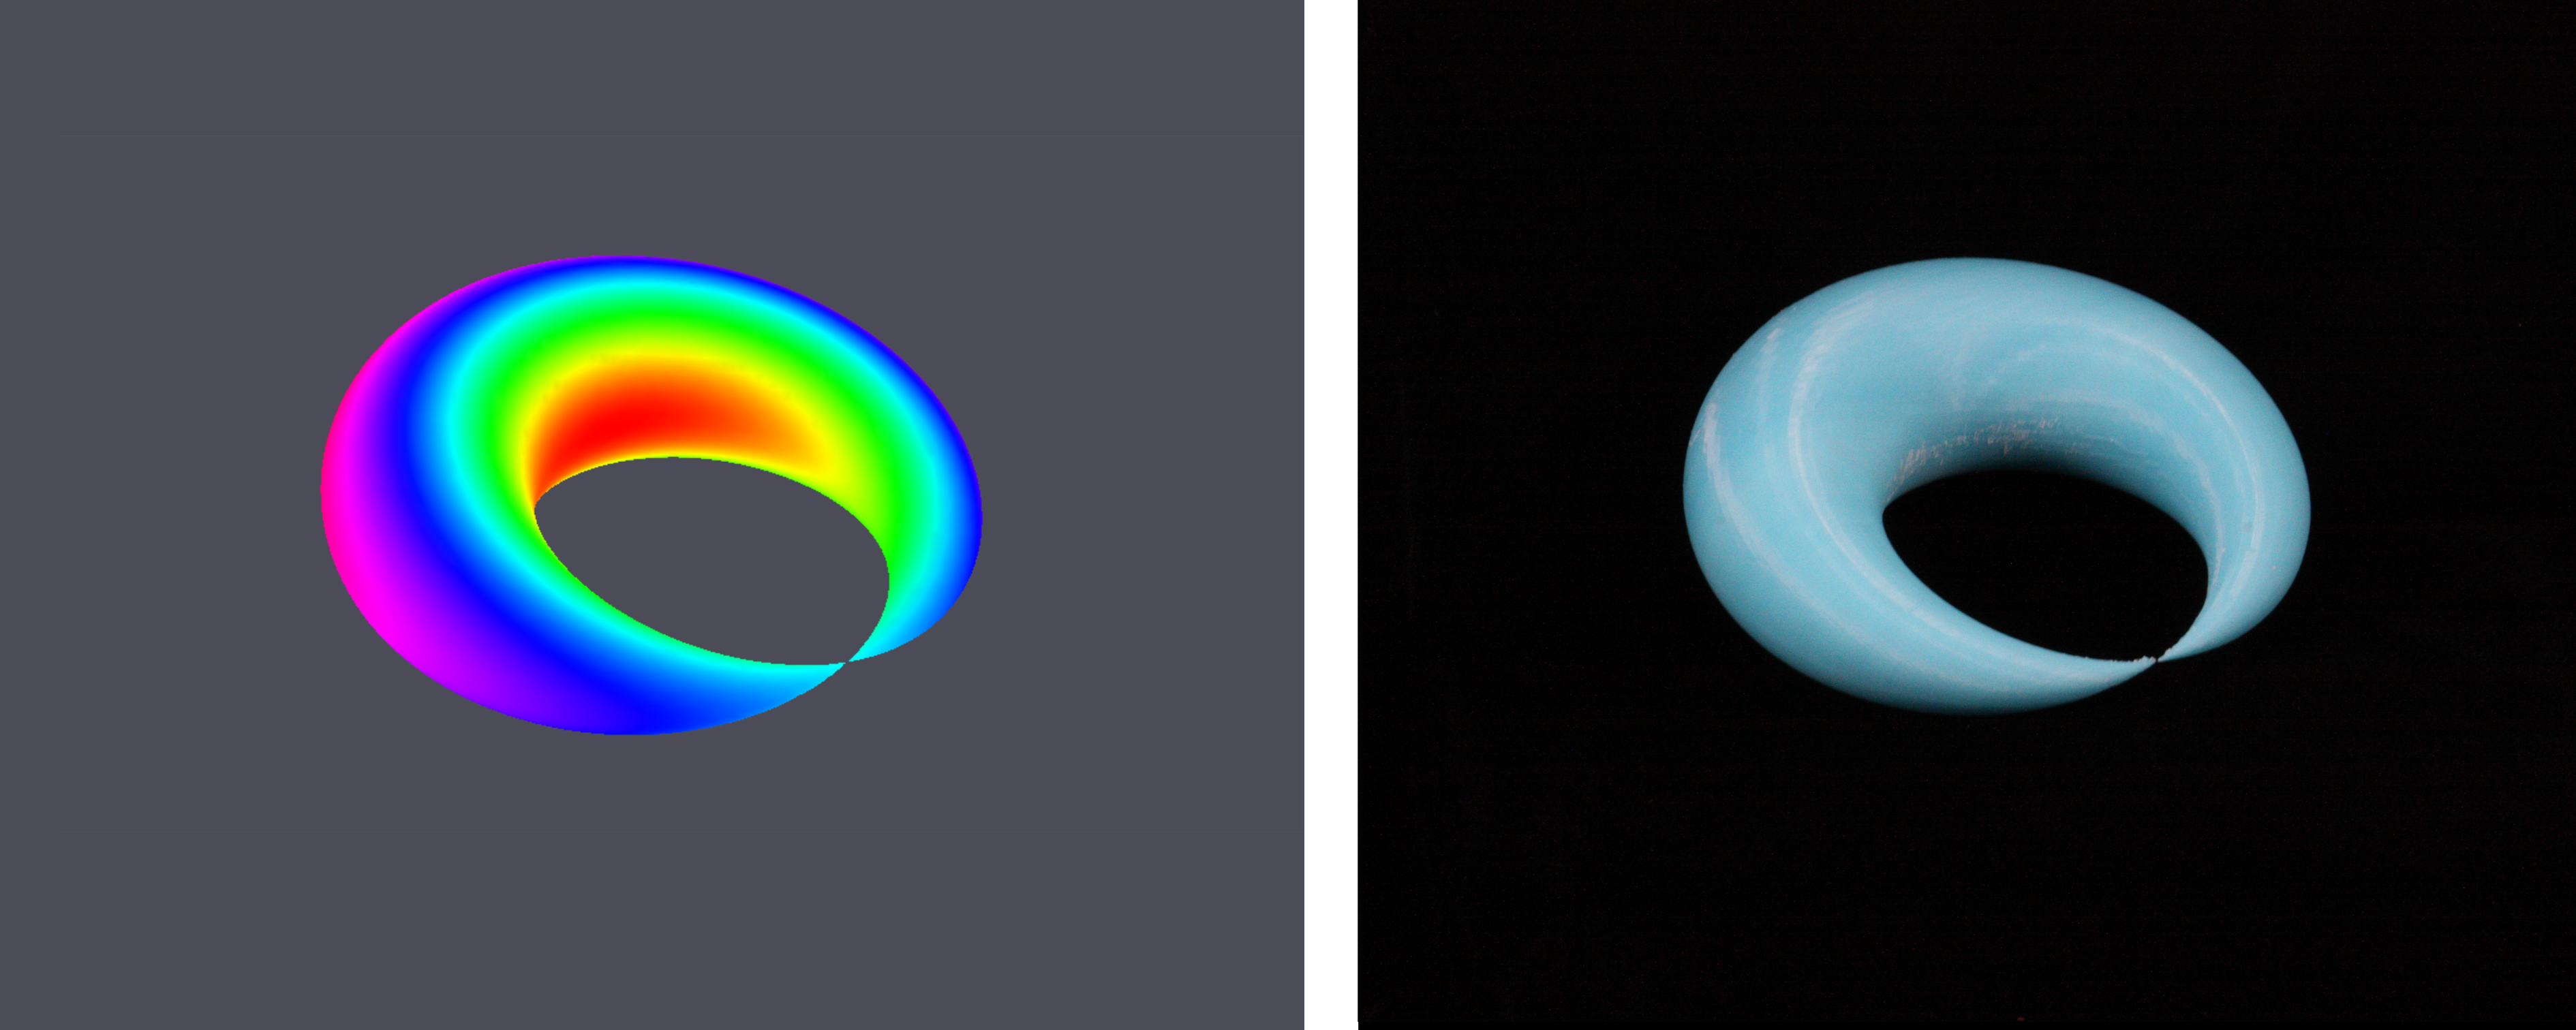
\includegraphics[width=2.10\linewidth, center]{pictures/croissant_ink.png}
    \end{center}
\end{minipage}

\vspace{5.2mm}

\begin{minipage}{0.95\linewidth}
The goal of our research was to use the open-source programming language Python to provide
new functionality to the free software program Bertini\_real. Bertini\_real has been using Matlab for surface
visualization; however, most students do not have the license to use it. Therefore, we aim to create Python-
based Bertini\_real visualization routines, that will provide free educational access for students.

\end{minipage}
\end{center}

}



\headerbox{Challenges \& future work}{name=challenges, column = 0, row = 0,span=2,below=goals}{ 

\vspace{1mm}

\begin{center}
\begin{minipage}[t]{0.90\linewidth}
We faced several challenges during the feature implementation process: 
\vspace{1mm}
\small
\begin{itemize}
\item \parbox[t]{\dimexpr\textwidth-\leftmargin}{%
Learn how to use Glumpy, a Python library, to plot and render 3D surfaces created from Bertini\_real
}
\vspace{1mm}
\item \parbox[t]{\dimexpr\textwidth-\leftmargin}{%
Research Python libraries such as Numpy-stl and Trimesh to export raw and sampler surface data correctly to stereolithography (STL)  for 3D printing 
}
\vspace{1mm}
\item \parbox[t]{\dimexpr\textwidth-\leftmargin}{%need to edit, more specfifc
Switch from OpenMesh to Numpy-stl and Trimesh to fix broken STLs with missing faces and surface normals 
}

\end{itemize}



\vspace{4mm}
Future work:
\small
\begin{itemize}
\item \parbox[t]{\dimexpr\textwidth-\leftmargin}{%
         Implement critical curve plot feature 
}
\item \parbox[t]{\dimexpr\textwidth-\leftmargin}{%
          Add a solidify feature to create offset surfaces
}
\end{itemize}

\vspace{4mm}
\begin{minipage}[t]{0.48\linewidth}
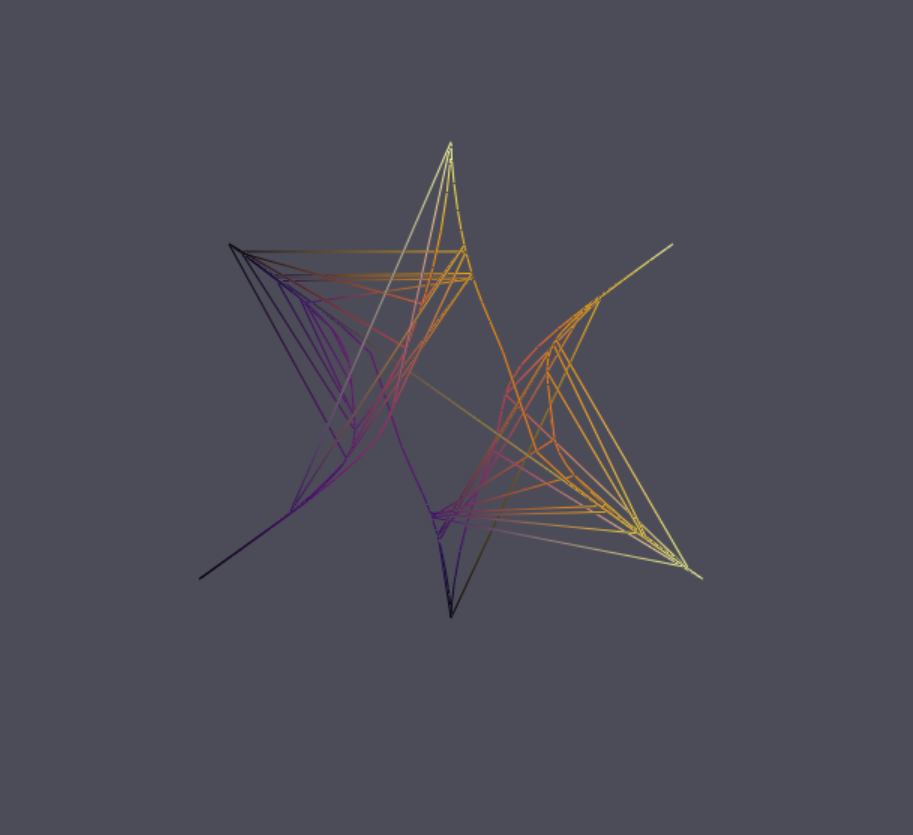
\includegraphics[width=1.05\linewidth,height= 0.80\linewidth]{pictures/fail_crit_curve}
\begin{center}

Broken critical curve
\end{center}

\end{minipage}
\hspace{0.01\linewidth}
\begin{minipage}[t]{0.48\linewidth}
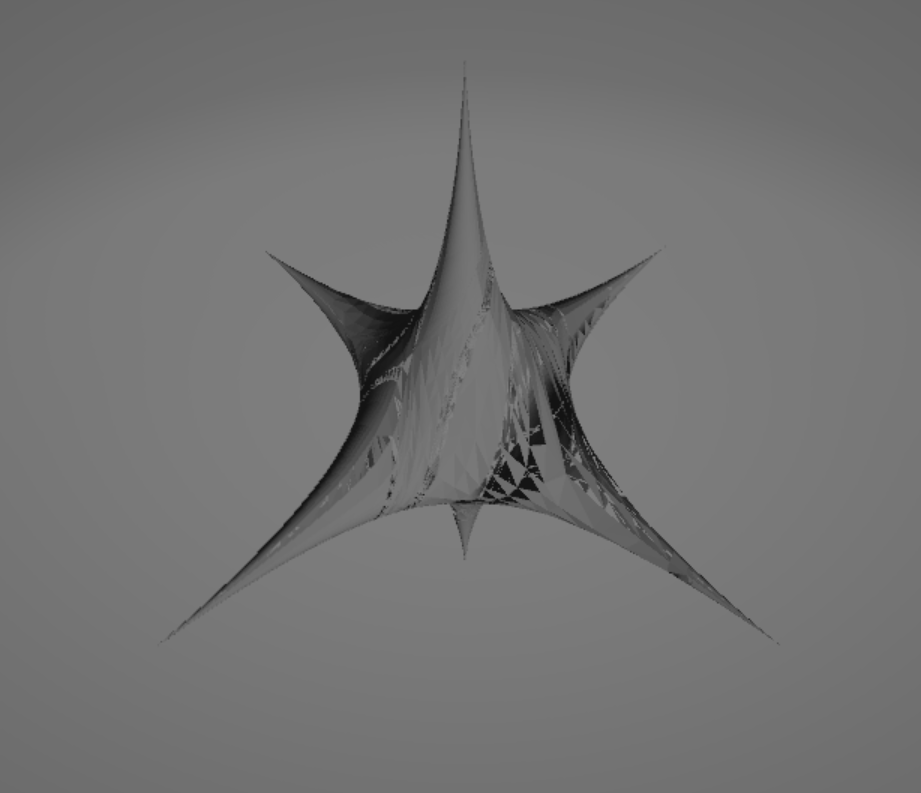
\includegraphics[width=1.05\linewidth ,height= 0.80\linewidth]{pictures/fail_stl}
\begin{center}

Broken STL
\end{center}

\end{minipage}


\normalsize


\end{minipage}
\vspace{1mm}


\end{center}



}



%%%%%%%%%
%%
%%  end of first column of boxes
%%
%%%%%%%%%%


%% this is a test ;D

\headerbox{3D Plots of Algebraic Surfaces}{name=printing, column=2, span=3}{
\begin{center}

\begin{minipage}[t]{0.48\linewidth}
    \begin{center}
        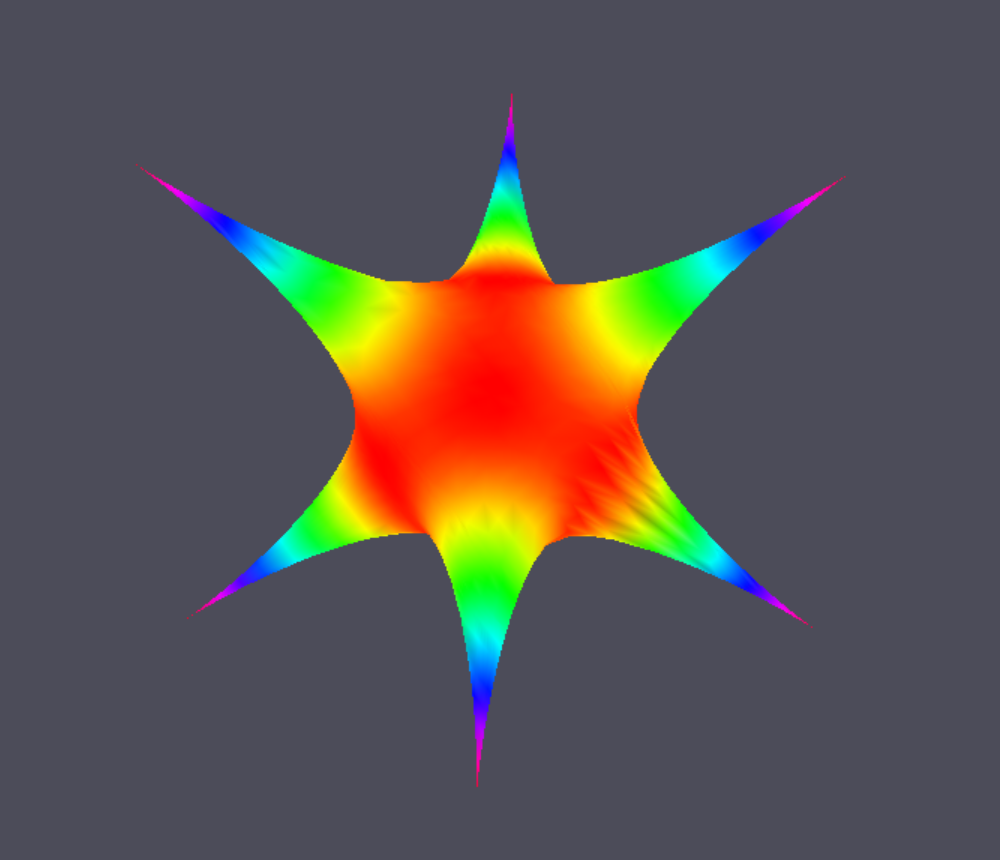
\includegraphics[width=.99\linewidth]{pictures/stern_crop}
        \vspace*{-7mm}
        \begin{gather*}
               \textnormal{Stern}\\
        400(x^2y^2+y^2z^2+x^2z^2)+\\(x^2+y^2+z^2-1)^3=0
        \\
        \end{gather*}
    \end{center}
\end{minipage}
% no space between boxes
\hspace{0.01\linewidth}
% no space between boxes
\begin{minipage}[t]{0.48\linewidth}
    \begin{center}
        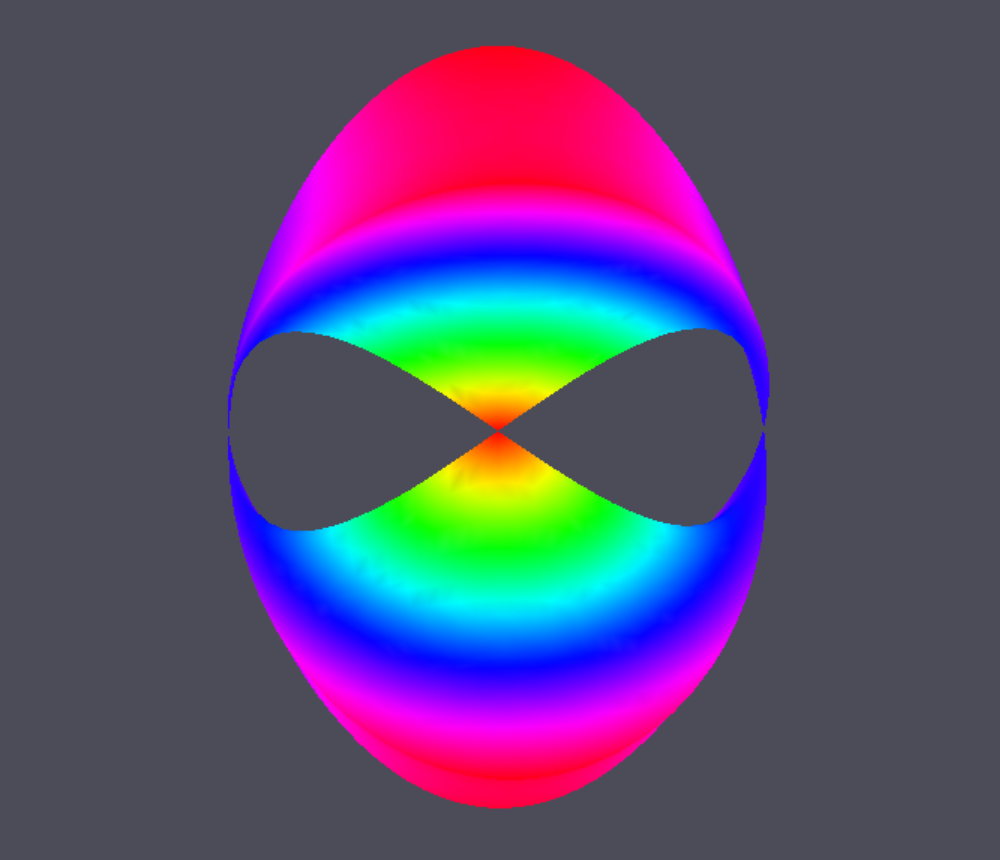
\includegraphics[width=.99\linewidth]{pictures/crixxi_crop}
        \vspace*{-7mm}
        \begin{gather*}
           \textnormal{Crixxi}\\
        (x^2+y^2+-1)^3+\\(y^2+z^2-1)^2=0
        \\
        \end{gather*}
    \end{center}
\end{minipage}
    \end{center}
}%%end of the header box 


\headerbox{3D Prints of Algebraic Surfaces}{name=plots, column=2 ,span=3,below=printing}{
\begin{center}
\begin{minipage}[t]{0.48\linewidth}
    \begin{center}
        \includegraphics[width=1.99\linewidth, center,trim={0cm 20cm 5cm 24cm},clip]{pictures/raw3_rotate}
        \vspace*{-7mm}
        \begin{gather*}
            \textnormal{Raw Version}
        \end{gather*}
        \end{center}
\end{minipage}

\vspace{3.0mm}

\begin{minipage}[t]{0.48\linewidth}
    \begin{center}
        \includegraphics[width=1.99\linewidth, center,trim={0 20cm 0 23cm},clip]{pictures/smooth3_rotate}
        \vspace*{-7mm}
        \begin{gather*}
            \textnormal{Smooth Version}
        \end{gather*}
        \end{center}
\end{minipage}
\end{center}
}%%end of the header box 




%%%%%%%%%%%%%%%
%%
%%  end of middle column
%%
%%%%%%%%%%%%%

\headerbox{Process}{name=process, column=5, row=0,span=2}{ %top

\begin{center}
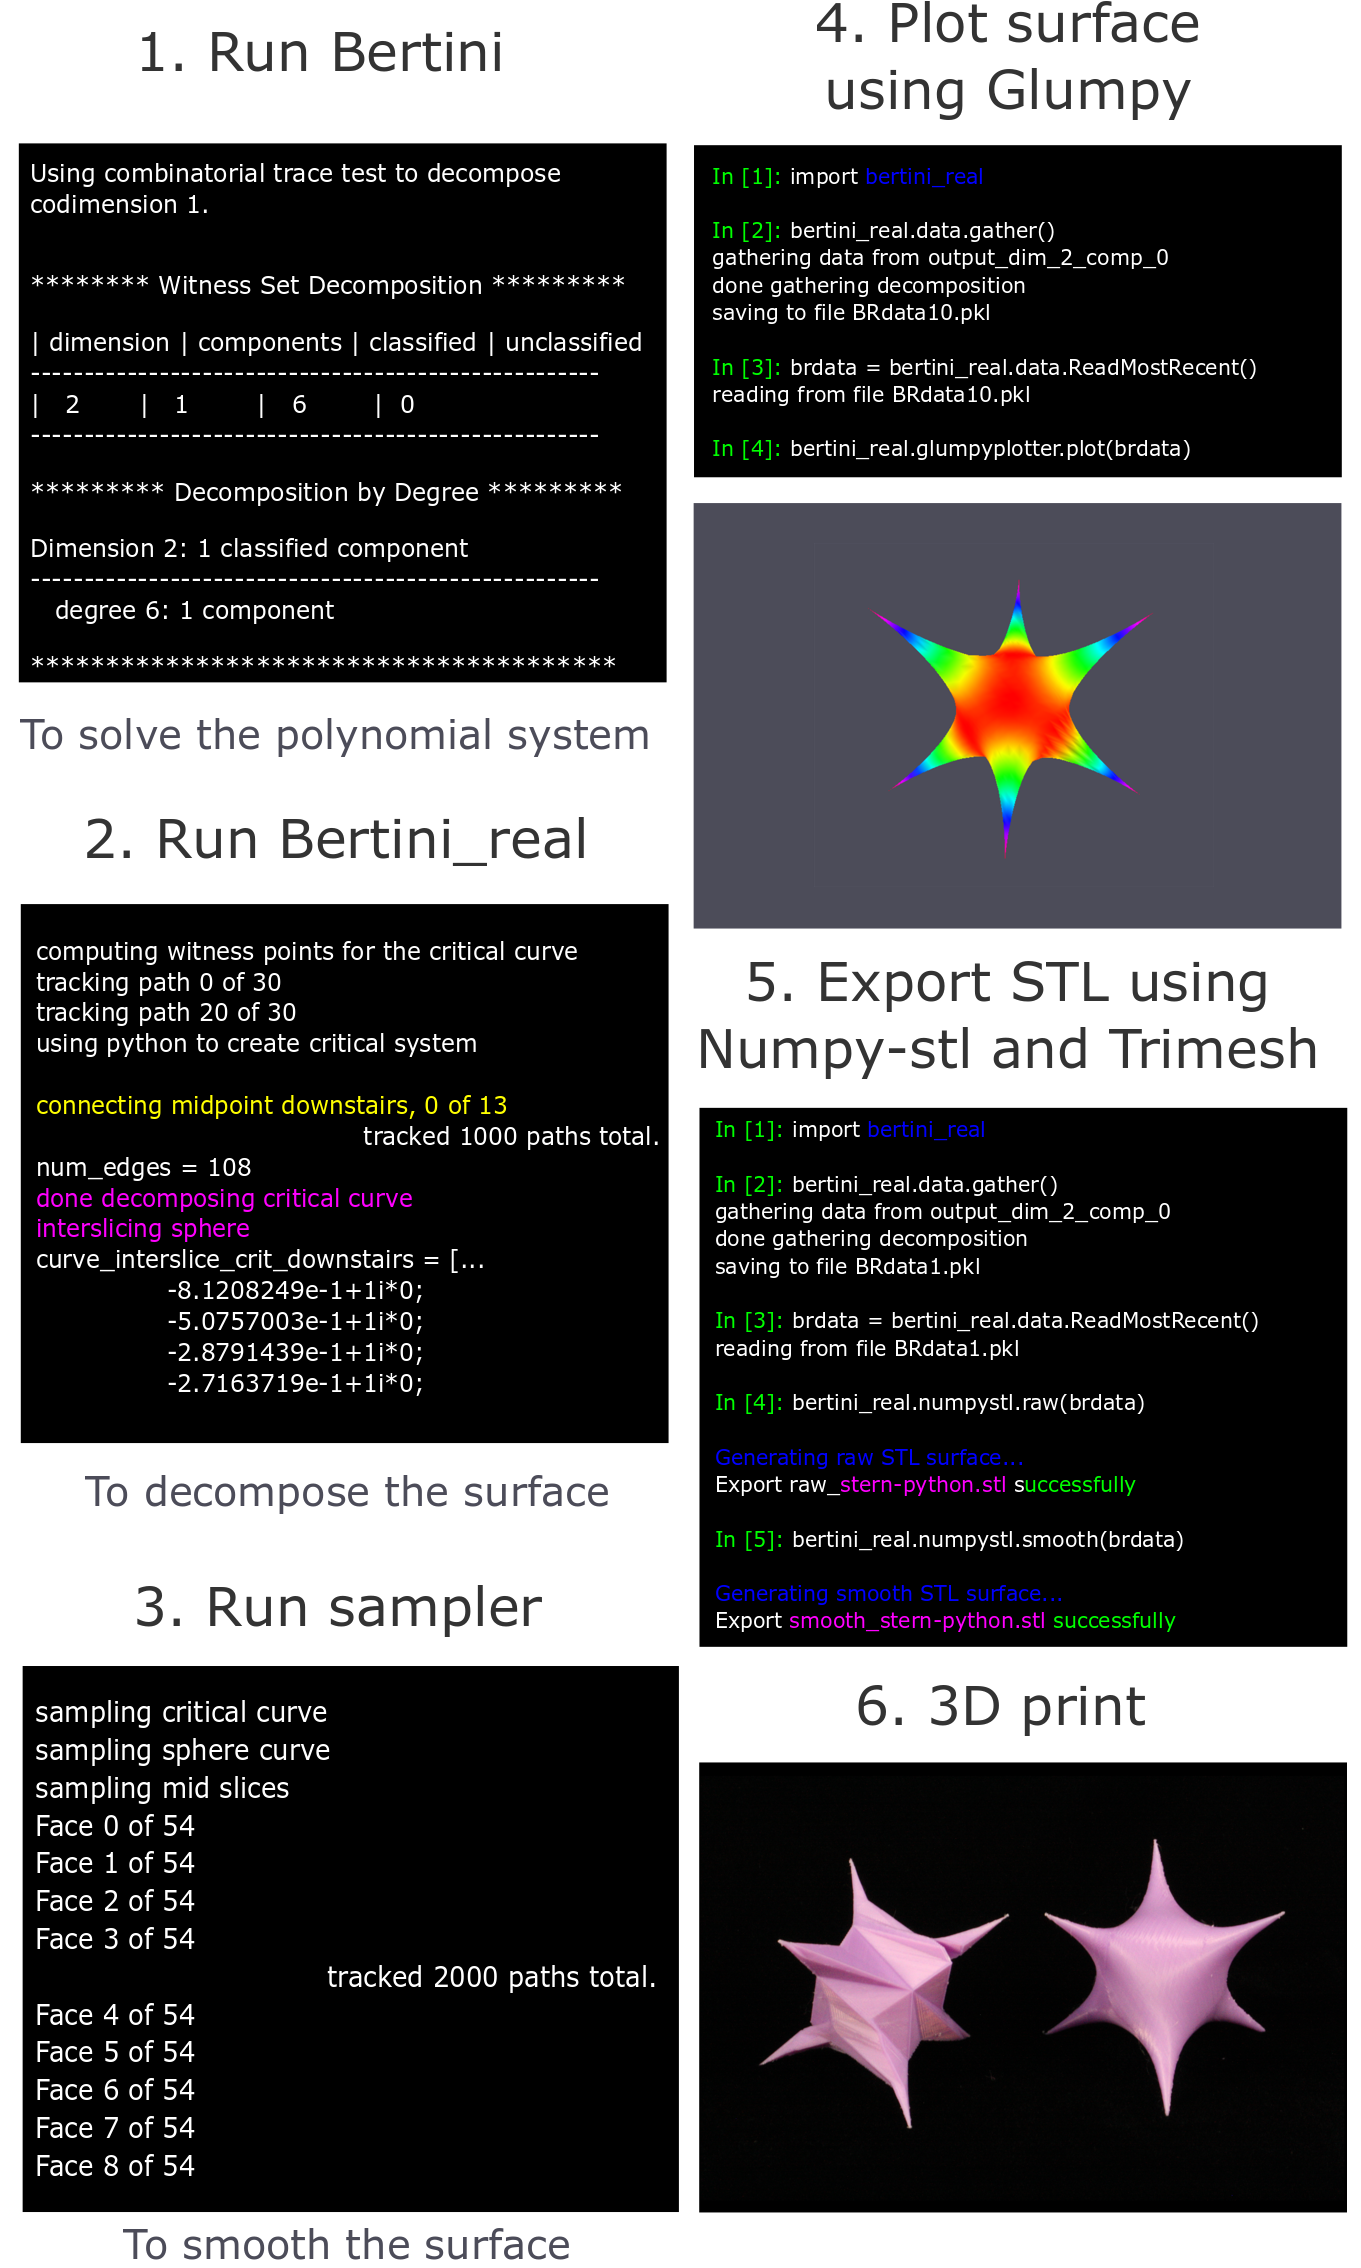
\includegraphics[width = \linewidth ]{pictures/process2.png}

\end{center}

}



\headerbox{References and acknowledgements}{name=references, column=5, below=process, span=2}{
\footnotesize													% Make the whole text smaller
\vspace{-0.4em} 									% Save some space at the beginning
\bibliographystyle{plain}							% Use plain style
\renewcommand{\section}[2]{\vskip 0.05em}		% Omit "References" title
\begin{thebibliography}{1}					% Simple bibliography with widest label of 1
\itemsep=0.235em									% Save space between the separation
\setlength{\baselineskip}{-0.5em}%0.2em  another spacing adjustment.

\bibitem{algebraicsurfacegallery}
H.~Hauser and J.~Schicho, ``Algebraic surfaces,'' 2014.
  \url{homepage.univie.ac.at/herwig.hauser/bildergalerie/gallery.html}

% \bibitem{Bertini}
% D.~J. Bates, J.~D. Hauenstein, A.~J. Sommese, and C.~Wampler, ``Bertini:
%   Software for numerical algebraic geometry,'' 2006-2018. 
%   \url{bertini.nd.edu}

\bibitem{BertiniReal}
D.~A. Brake, D.~J.~Bates, W.~Hao, J.~D. Hauenstein, A.~J. Sommese, and
  C.~W. Wampler, ``Algorithm 976: Bertini\_real: Numerical decomposition of
  real algebraic curves and surfaces,'' \emph{ACM Transactions on Mathematical
  Software (TOMS)}.

\vspace{6.3mm}	
This project received generous support from Office of Research and Sponsored Programs Faculty and Undergraduate Student Research Collaboration, and Learning and Technology Services. 
\end{thebibliography}


}


%%%%%%%%%%%%%%%
%%
%%  end of last column
%%
%%%%%%%%%%%%%


\end{poster}
\end{document} 




